\documentclass[conference]{IEEEtran}
\IEEEoverridecommandlockouts
\usepackage{cite}
\usepackage{amsmath,amssymb,amsfonts}
\usepackage{algorithmic}
\usepackage{graphicx}
\usepackage{textcomp}
\usepackage{xcolor}
\usepackage{booktabs}
\usepackage{tabularx}

\def\BibTeX{{\rm B\kern-.05em{\sc i\kern-.025em b}\kern-.08em
    T\kern-.1667em\lower.7ex\hbox{E}\kern-.125emX}}
\begin{document}

\title{Decentralized Swarm Autonomy Framework for Cyber-Physical Systems under Communication and Energy Constraints\\
\thanks{Identify applicable funding agency here. If none, delete this.}
}

\author{\IEEEauthorblockN{1\textsuperscript{st} Shivam Malge}
\IEEEauthorblockA{\textit{Dept. of Computer Science} \\
\textit{(Data Science)}\\
\textit{Atria Institute Of Technology}\\
Bangalore, India \\
shivammalge@gmail.com}
\and
\IEEEauthorblockN{2\textsuperscript{nd} Prajwal Narendra Hegde}
\IEEEauthorblockA{\textit{Dept. of Computer Science} \\
\textit{(Data Science)}\\
\textit{Atria Institute Of Technology}\\
Bangalore, India \\
prajwalhegde3010@gmail.com}
\and
\IEEEauthorblockN{3\textsuperscript{rd} Koushik K R}
\IEEEauthorblockA{\textit{Dept. of Computer Science} \\
\textit{(Data Science)}\\
\textit{Atria Institute Of Technology}\\
Bangalore, India \\
koushik.kr.2004@gmail.com}
\and
\IEEEauthorblockN{4\textsuperscript{th} Ms. Shruthi}
\IEEEauthorblockA{\textit{Dept. of Information Science Engineering} \\
\textit{Atria Institute of Technology}\\
Bengaluru, India \\
shruthi@atria.edu | ORCID: 0000-0001-9876-5432}
}

\maketitle

\begin{abstract}
Decentralized swarm autonomy requires agents to coordinate under unreliable communication, partial observability, and irreversible energy depletion. This paper presents a modular, event-driven simulation framework for decentralized drone swarms that enforces strict fog-of-war constraints: agents operate exclusively on stale neighbor beliefs maintained in local maps, with no access to global topology. The simulation kernel implements a deterministic discrete event model with independent random number streams, ensuring reproducible execution. Inter-agent communication is modeled as a stochastic Random Geometric Graph with Bernoulli packet drops. Three distributed coordination algorithms---gossip-based consensus, localized Voronoi coverage, and auction-based task allocation---execute solely on local information. A passive regime detection layer classifies the environment into operational states, driving a hybrid supervisor that proposes parameter adjustments. These updates pass through a control pipeline utilizing a local bisection search and exponential moving average smoothing. Stress testing with 100 agents over 15 million discrete events demonstrates sustained network connectivity, demonstrating quadratic per-transmission energy scaling that empirically yields a stable, linear aggregate decay trajectory under 50\% node attrition, and smooth adaptive parameter evolution with mean per-update shifts empirically bounded below 0.04. The framework accurately evaluates necessary local heuristic relaxations of classical control theorems under severe communication constraints.\footnote{The complete simulation kernel, baseline configurations, and execution scripts are open-source: \texttt{https://github.com/ShivamMalge/swarm\_drone\_framework}}
\end{abstract}

\section{Introduction}

The expansion of multi-agent robotics has significantly influenced the operational capabilities of autonomous systems in contested environments. By eliminating single points of failure, decentralized drone swarms offer a resilient approach to complex spatial operations [8], [23]. In modern cyber-physical system (CPS) deployments, individual drones act as independent nodes tasked with maintaining spatial coverage, reaching consensus, and executing distributed task auctions [1], [9]. However, the decentralized nature of these flows introduces challenges regarding structural connectivity, energy management, and behavioral stability when operating under severe epistemic uncertainty [2].

Current multi-agent simulation frameworks often rely on assumptions that do not fully reflect the constraints of physical deployment [3], [22]. A notable gap in the existing literature is the widespread reliance on continuous-time feedback loops and zero-latency communication graphs. Furthermore, many simulated environments inadvertently allow agents to access global state arrays, violating strict "Fog-of-War" constraints. When algorithms developed under these assumptions are deployed onto physical hardware, they are susceptible to severe failure modes triggered by unpredictable packet dropping and topological fragmentation. Moreover, traditional frameworks frequently abstract away thermodynamic energy constraints, which can lead to inverse energy cascades as node depletion forces surviving neighbors to expend exponentially more energy [22].

Addressing these vulnerabilities requires transitioning from perfect-information models to discrete-event architectures that enforce partial observability. As swarms rely on adaptive heuristic parameters to navigate changing regimes, there is a critical need to ensure that such mutations do not violate the closed-loop stability of the network. Without mathematical bounds, unconstrained adaptation often induces kinematic oscillations and network fracturing.

To bridge this gap, this paper introduces a Decentralized Swarm Autonomy Framework designed as an engineering testbed for contested cyber-physical environments. Rather than claiming fundamental mathematical novelty, this approach emphasizes engineering realism: it tightly couples thermodynamic energy constraints with epistemic Fog-of-War limitations (RGG with stochastic packet drops), and bounds the swarm's behavioral adaptation using a localized stability-constrained bisection search. By departing from legacy continuous-time models and employing a deterministic Discrete-Event Simulation (DES) environment, the framework provides a highly realistic platform to evaluate how localized heuristic relaxations of centralized control theorems can maintain connectivity and avert catastrophic cascading failures without centralized oversight.

The primary contributions are:
\begin{enumerate}
 \item \textbf{Enforced Fog-of-War:} A simulation framework where agents rely exclusively on stale, asynchronous neighbor data to execute coverage, consensus, and sequential single-item (SSI) auctions.
 \item \textbf{Passive Regime Detection:} A distributed telemetry buffer that allows agents to autonomously classify their environmental state using locally computable proxy metrics.
 \item \textbf{Stability-Constrained Adaptation:} A control pipeline applying iterative bisection searches against local stability boundaries to constrain heuristic adaptation, mitigating kinematic divergence.
 \item \textbf{Deterministic Reproducibility:} A discrete-event architecture driven by independent random number streams, enabling exact replay of stochastic failures.
\end{enumerate}

To highlight the novelty of this approach, Table \ref{tab:comparison} compares the proposed framework against archetypal methodologies in multi-agent coordination.

\begin{table}[htbp]
\caption{Comparison of Multi-Agent Coordination Paradigms}
\begin{center}
\begin{tabularx}{\linewidth}{@{}l*{4}{>{\centering\arraybackslash}X}@{}}
\toprule
\textbf{Methodology} & \textbf{Fog-of-War Modeling} & \textbf{Epistemic Boundary} & \textbf{Energy Constraints} & \textbf{Safe Adaptation} \\
\midrule
Continuous Flocking [5] & No & No & No & No \\
Centralized Coverage [14] & No & No & Yes & No \\
Unconstrained RL & Yes & Yes & Yes & No \\
\textbf{Proposed Framework} & \textbf{Yes} & \textbf{Yes} & \textbf{Yes} & \textbf{Yes} \\
\bottomrule
\end{tabularx}
\label{tab:comparison}
\end{center}
\end{table}

\section{Background and Related Work}

In cyber-physical systems (CPS), achieving decentralized autonomy improves the survivability and scalability of multi-agent swarms. The engineering of such systems requires a synthesis of distributed control theory, stochastic network physics, and spectral graph analysis [1], [6]. To contextualize our contributions, Table \ref{tab:comparison_lit} compares our approach against foundational methodologies across critical engineering constraints.

\begin{table}[htbp]
\caption{Comparison of Multi-Agent Frameworks}
\begin{center}
\begin{tabularx}{\linewidth}{@{}l*{6}{>{\centering\arraybackslash}X}@{}}
\toprule
\textbf{Work} & \textbf{Consensus} & \textbf{Energy} & \textbf{Packet Loss} & \textbf{Fog-of-War} & \textbf{DES} & \textbf{Auctions} \\
\midrule
Olfati-Saber [1] & \checkmark & X & X & X & X & X \\
Cort\'{e}s [2] & X & X & X & X & X & X \\
Yang [6] & \checkmark & X & X & X & X & X \\
SwarmFly [9] & \checkmark & \checkmark & \checkmark & Partial & X & X \\
\textbf{This Work} & \textbf{\checkmark} & \textbf{\checkmark} & \textbf{\checkmark} & \textbf{\checkmark} & \textbf{\checkmark} & \textbf{\checkmark} \\
\bottomrule
\end{tabularx}
\label{tab:comparison_lit}
\end{center}
\end{table}

\subsection{Distributed Consensus \& Multi-Agent Coordination}
Consensus algorithms are fundamental to multi-agent coordination [1], [5], [19]. Foundational work by Olfati-Saber and Murray [1] establishes convergence for networks with time-delays, while subsequent research has extended these principles to asynchronous gossip protocols and quantized communication [19]. Existing work typically assumes mathematically rigorous convergence under specific communication assumptions. In contrast, our work explicitly focuses on engineering robustness under severe packet loss and strictly localized information [12], [15], [17], accepting heuristic relaxations to preserve operational stability in contested kill webs [24].

\subsection{Task Allocation and Voronoi Coverage}
Distributing spatial coverage relies heavily on localized geometric partitioning, extending Lloyd-descent algorithms to adaptive and minimum-energy coverage paradigms [10], [18]. To assign discrete tasks within these continuous territories, swarms leverage bidding mechanisms such as Sequential Single-Item (SSI) auctions and submodular optimization [4], [21]. In communication-constrained environments, these allocations must execute entirely over asynchronous gossip protocols based on spatial risk and remaining energy margins [11].

\subsection{Connectivity Maintenance}
Maintaining algebraic connectivity ($\lambda_2$) is critical for swarm cohesion [6], [13]. Existing approaches estimate or preserve algebraic connectivity using distributed eigenvalue estimation, decentralized power iteration, or continuous gradient descent [6], [13]. Our framework intentionally avoids these bandwidth-intensive methods. Instead, it employs an empirical local mixing proxy suitable for severe communication constraints. Rather than claiming our method is strictly better, our design makes a different engineering trade-off: trading exact global estimation for low-latency, localized heuristic approximation.

\subsection{UAV Swarm Energy Models}
Energy depletion dictates the lifespan of a deployed swarm [7], [22]. Prior work by Wu et al. [7] and others focuses heavily on optimizing UAV trajectories and continuous communication energy. Our simulator diverges by studying how communication degradation and discrete energy depletion jointly reshape swarm connectivity over time. We model thermodynamic decay as a primary driver of topological alterations, triggering inverse energy cascades as surviving nodes compensate for attrition [16].

\subsection{Swarm Simulation Platforms}
Robotic simulation relies heavily on continuous-time platforms such as ROS2, Gazebo, ARGoS, and specialized frameworks like CrazySwarm or SwarmFly [9]. Existing simulators provide high-fidelity continuous physics and kinematic realism, but are computationally expensive for rapid, large-scale algorithmic experimentation. Our lightweight Discrete-Event Simulation (DES) framework emphasizes deterministic reproducibility and communication-layer experimentation over aerodynamic fidelity.

\subsection{Research Gap}
Existing work typically investigates consensus, connectivity maintenance, energy-aware communication, and swarm simulation independently. This work integrates these aspects within a deterministic discrete-event framework operating under strict local epistemic constraints, enabling reproducible evaluation of decentralized swarm behaviors under severe communication degradation.

\section{Decentralized System Methodology and Simulation}

To translate this framework into a highly reproducible execution environment, the system is engineered using a modular design. The architecture explicitly separates the physical simulation physics from the decentralized agent logic, enabling event-driven evaluation while ensuring interoperability with embedded control systems.

\subsection{Decentralized Agent Architecture}
The system is partitioned to enforce a strict epistemic boundary (``Fog-of-War''). As illustrated in Figure \ref{fig:arch}, the architecture consists of two primary layers:
\begin{itemize}
    \item \textbf{Discrete-Event Simulation (DES) Environment:} Acts as the deterministic ground truth. It manages the global coordinate space, evaluates the stochastic Random Geometric Graph (RGG) communication physics, and computes the monotonic thermodynamic energy decay for all entities.
    \item \textbf{Distributed Intelligence Subsystem:} Encapsulates the agent logic. It houses the Local Belief Buffer, the Asynchronous Gossip Protocol handler, and the stability-constrained bisection pipeline. This module has absolutely zero access to the DES global state; it strictly processes delayed telemetry received through simulated network interfaces.
\end{itemize}

\begin{figure}[htbp]
    \centering
    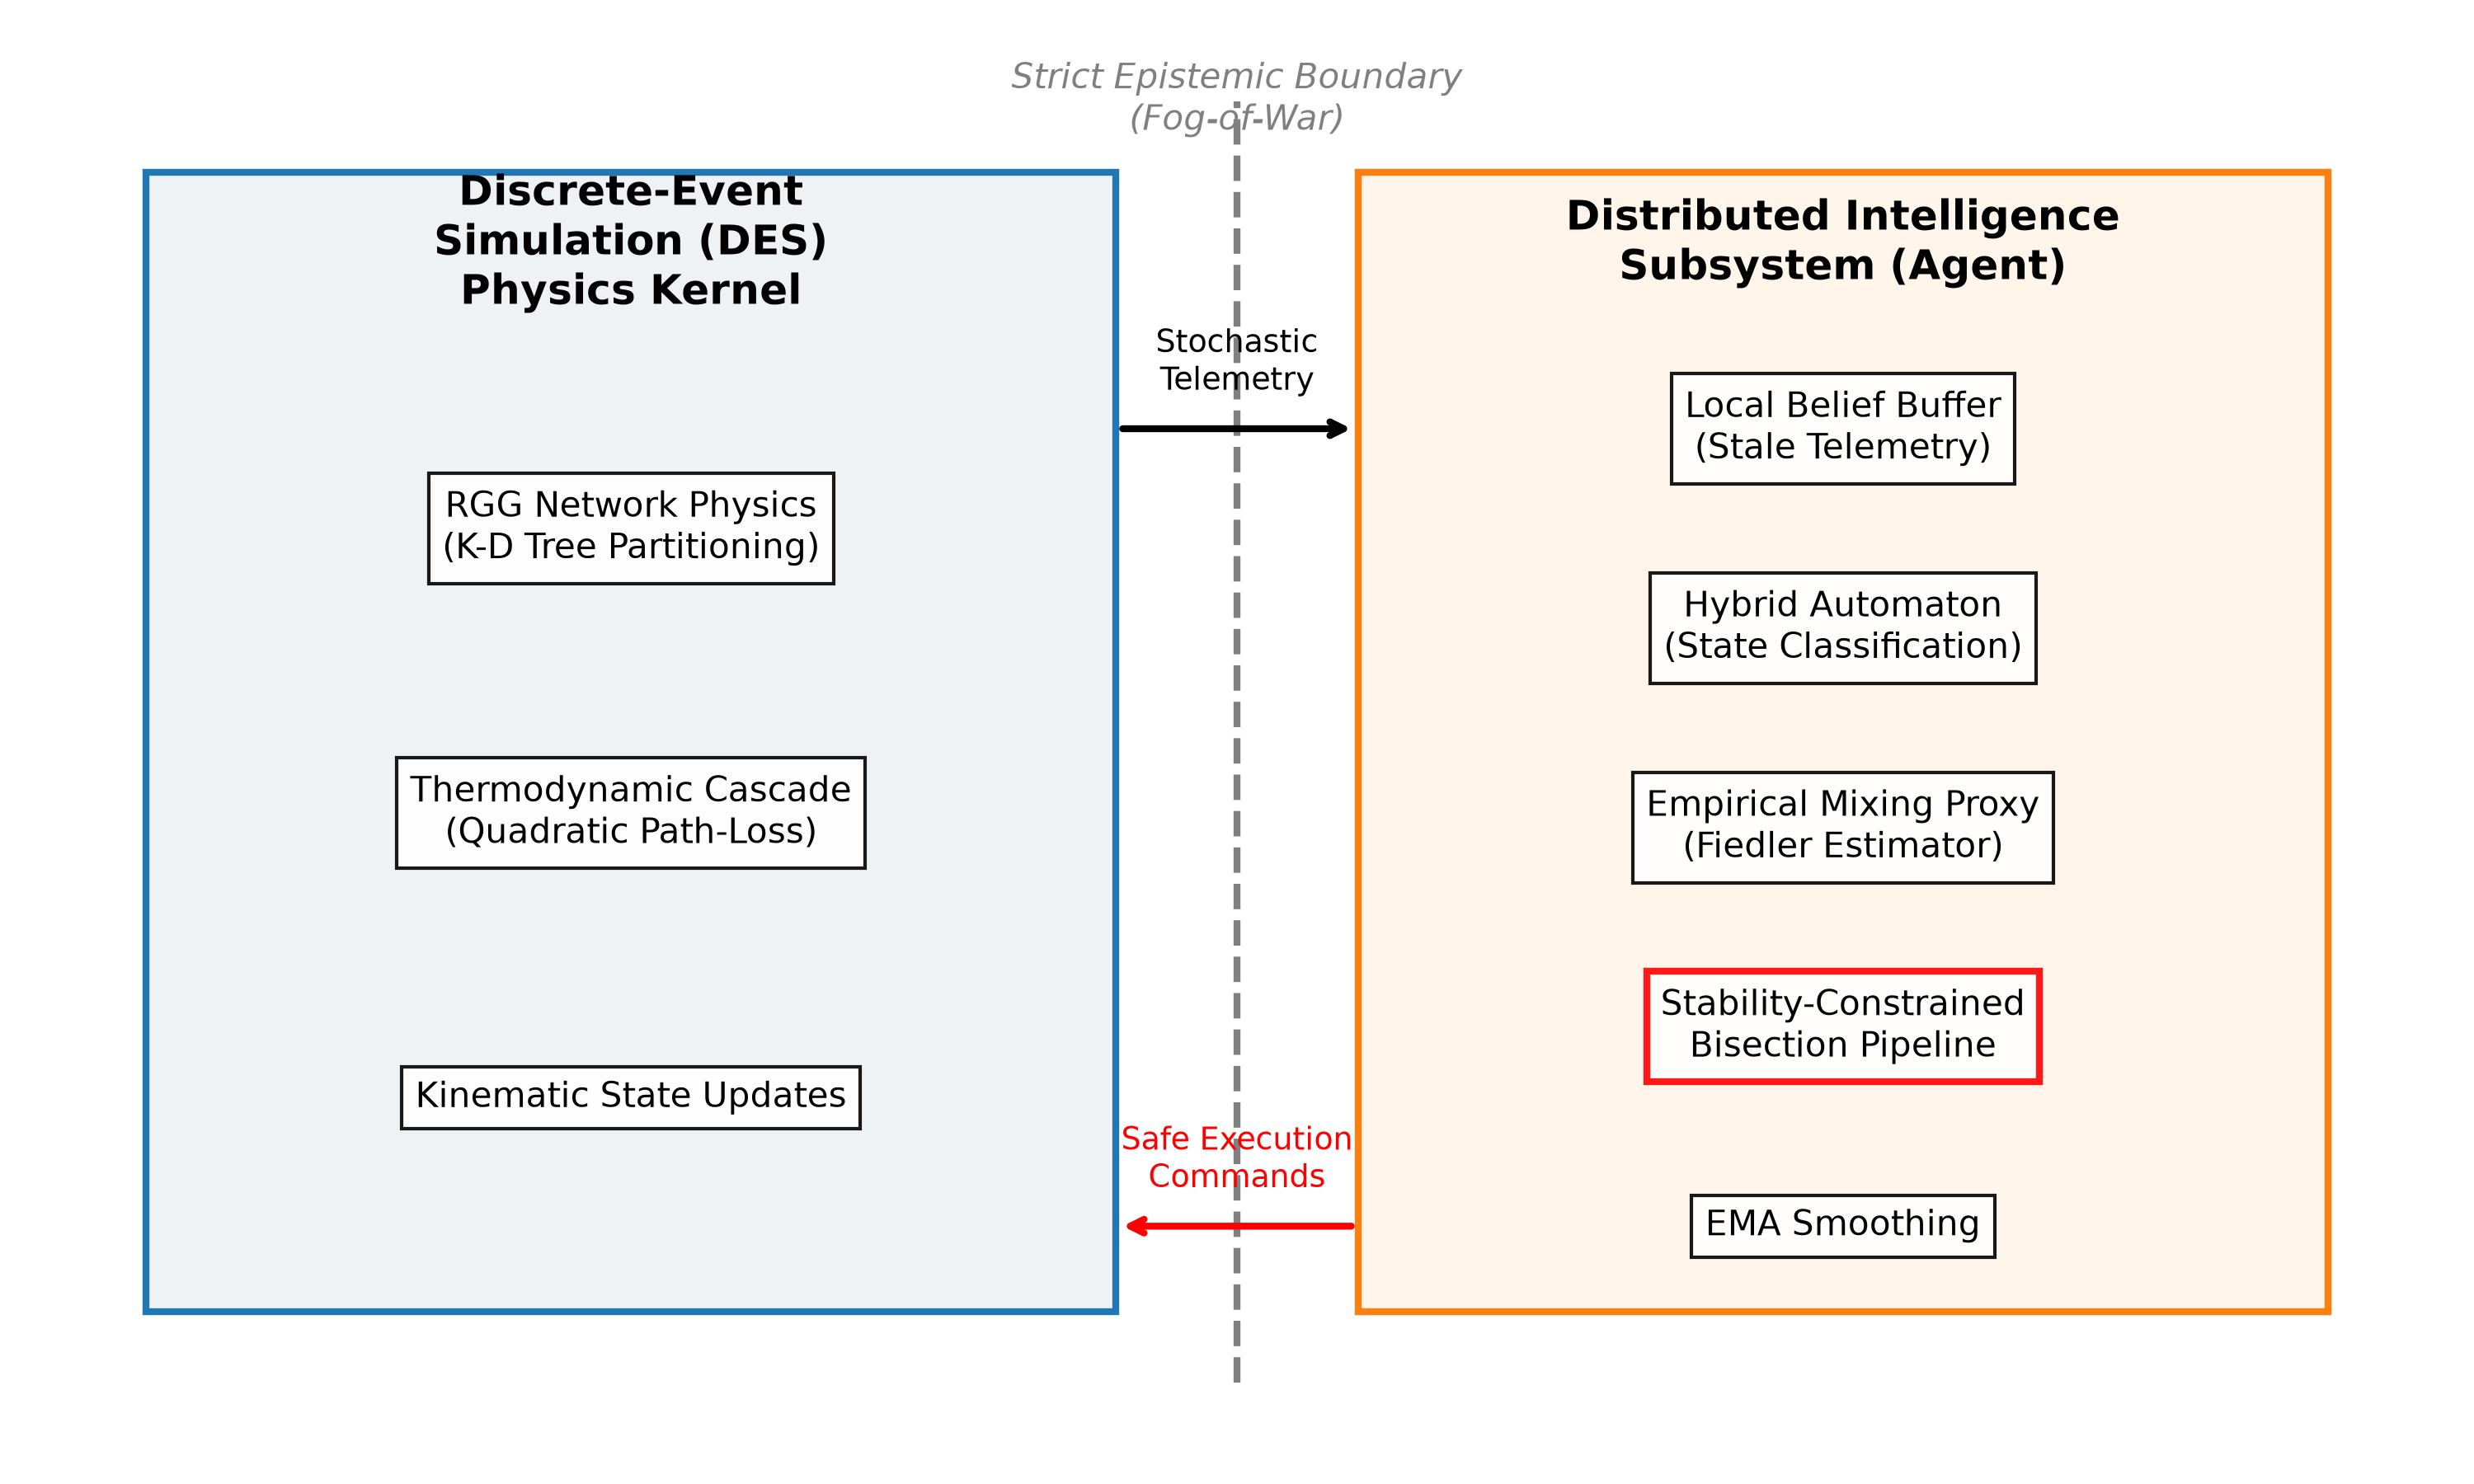
\includegraphics[width=\linewidth]{fig4_architecture.png}
    \caption{High-Level System Architecture detailing the discrete-event physics layer and decentralized agent logic enforcing the epistemic boundary.}
    \label{fig:arch}
\end{figure}

The control flow operates on a discrete pipeline. Surviving telemetry packets flow into the agent's Distributed Intelligence Subsystem, updating the Local Belief Buffer. The Hybrid Supervisor evaluates local metrics and proposes a heuristic parameter mutation. Before execution, this raw proposal is intercepted by the Local Stability Projector, which mathematically bisects the vector against computed local stability boundaries. The safe execution commands are then passed to the DES Kernel to update physical reality.

\subsection{Discrete-Event Physics Pipeline}
To ensure reproducible evaluation of multi-agent dynamics, the simulation framework adheres to a chronological execution pipeline driven by a min-heap priority queue.
\begin{itemize}
    \item \textbf{Network Physics:} At the onset of each simulation tick ($t_k$), connectivity is evaluated through RGG construction, calculating Euclidean distances and signal-to-noise ratios. The kernel simulates delayed and stochastic packet propagation, filtering telemetry according to the RGG topology before injecting surviving packets into the Local Belief Buffers.
    \item \textbf{Epistemic Processing:} Agents conduct spatial task allocation using Decentralized SSI auctions, bidding based on immediate spatial risk and energy margins. Subsequently, agents compute localized metrics, feeding into the Hybrid Automaton which dictates autonomous regime shifts. To prevent chattering (rapid oscillatory switching between regimes), the supervisor strictly enforces a fixed Dwell Time ($\tau_d = 5.0$ ticks) before permitting subsequent transitions.
    \item \textbf{Physical Execution:} Verified action commands are executed. The kernel updates kinematic positions and immediately calculates thermodynamic energy updates, applying decay penalties associated with movement and transmission power. Agents whose energy falls below the critical threshold are culled from the simulation.
\end{itemize}

\subsection{Computational Scalability}
The architecture is designed to decouple the per-agent operational logic from the macroscopic swarm size ($N$). While dynamically updating the RGG adjacency matrix evaluates globally at $\mathcal{O}(N \log N)$ using K-D Tree spatial partitioning, all onboard intelligence layers scale locally. Distributed estimation, SSI auctions, and the Stability-Constrained Bisection Search execute in $\mathcal{O}(d)$ or $\mathcal{O}(1)$ time relative to the local neighborhood degree $d$. This architectural approach supports scalable deployment on constrained hardware in dense swarms.

\section{Mathematical Formulation and Algorithmic Flow}

The framework relies on a set of mathematical models and localized algorithms executed exclusively using delayed, asynchronous telemetry.

\subsection{Algorithmic Workflow}

\textbf{Algorithm 1: Bounded Heuristic Clamping} ensures that behavioral mutations triggered by the Hybrid Supervisor undergo an iterative bisection search, mitigating kinematic divergence by clamping parameters to heuristic thresholds. The data flow for this interception protocol is detailed in the sequence diagram in Figure \ref{fig:sequence}.

\begin{figure*}[htbp]
    \centering
    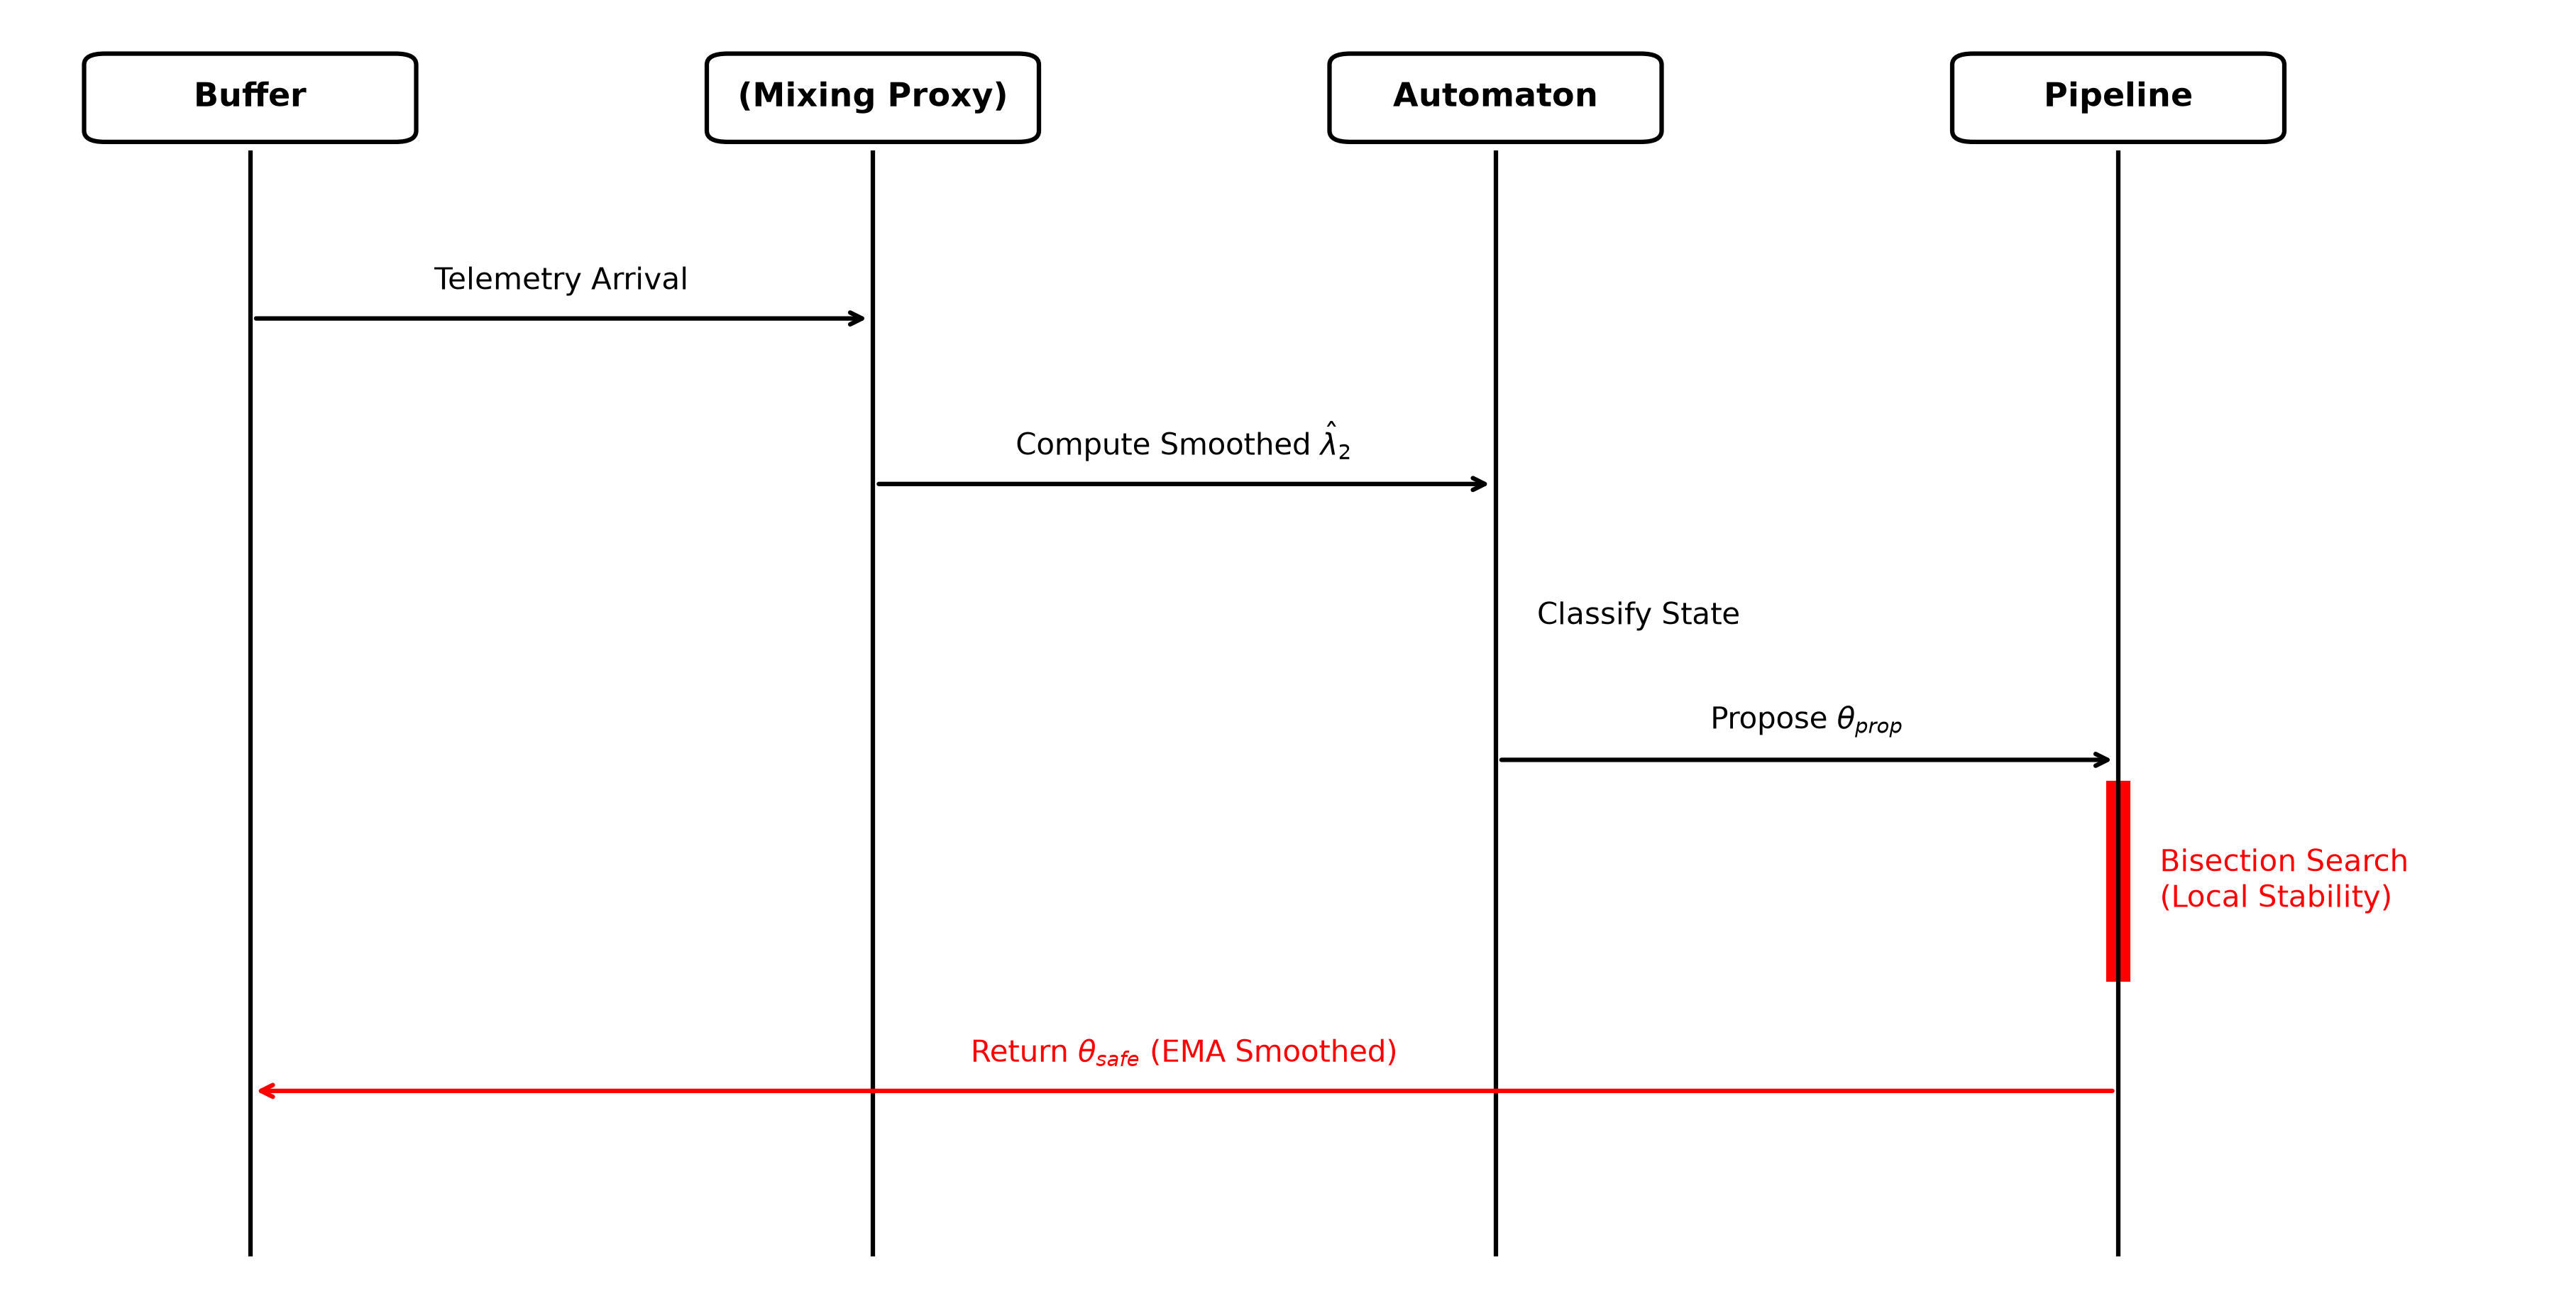
\includegraphics[width=\textwidth]{fig5_sequence.png}
    \caption{Sequence diagram mapping the data flow of the stability-constrained adaptation protocol. The local bisection projector acts as a heuristic saturation filter intercepting unconstrained proposals.}
    \label{fig:sequence}
\end{figure*}

\noindent \textbf{Algorithm 1: Bounded Heuristic Clamping} \\
\textbf{Input:} $\mathcal{T}_{buffer}$ (telemetry), $\theta_{curr}$ (current parameters), $\alpha$ (EMA coefficient), $\theta_{nominal}$ (baseline parameters), $\theta_{bounds}$ (one-directional safety thresholds) \\
\textbf{Precondition:} $\theta_{nominal} \le \theta_{bounds} \le \theta_{prop}$ \\
\textit{// Step 1: Epistemic State Classification} \\
$\mu_{local} \leftarrow \text{ComputeSmoothedAverages}(\mathcal{T}_{buffer})$ \\
$\text{Regime} \leftarrow \text{HybridSupervisor}(\mu_{local})$ \\
$\theta_{prop} \leftarrow \text{MapRegimeToStrategy}(\text{Regime})$ \\
\textit{// Step 2: Bounded Heuristic Clamping Search} \\
\textbf{for each} parameter $k$ in $\theta_{prop}$ \textbf{do} \\
\quad \textbf{if} $\theta_{prop}[k] \ge \theta_{bounds}[k]$ \textbf{then} \\
\quad \quad $low \leftarrow \theta_{nominal}[k]$, $high \leftarrow \theta_{prop}[k]$ \\
\quad \quad \textbf{for} $step = 1$ to $5$ \textbf{do} \\
\quad \quad \quad $mid \leftarrow (low + high) / 2$ \\
\quad \quad \quad \textbf{if} $mid < \theta_{bounds}[k]$ \textbf{then} $low \leftarrow mid$ \textbf{else} $high \leftarrow mid$ \\
\quad \quad \textbf{end for} \\
\quad \quad $\theta_{safe}[k] \leftarrow low$ \\
\quad \textbf{else} \\
\quad \quad $\theta_{safe}[k] \leftarrow \theta_{prop}[k]$ \\
\quad \textbf{end if} \\
\textbf{end for} \\
\textit{// Step 3: EMA Kinematic Smoothing} \\
$\theta_{next} \leftarrow \theta_{curr} + \alpha (\theta_{safe} - \theta_{curr})$ \\
\textbf{Return} $\theta_{next}$

\vspace{1em}

\noindent \textbf{Algorithm 2: Decentralized SSI Auction} prioritizes thermodynamic survivability and spatial efficiency while requiring communication only with immediate neighbors.

\vspace{0.5em}
\noindent \textbf{Algorithm 2: Decentralized SSI Auction} \\
\textbf{Input:} $T_{unasgnd}$ (unassigned tasks), $p_i$ (agent position), $E_i$ (remaining energy), $\Delta t_{auc}$ (auction duration) \\
$\mathcal{T}_{v} \leftarrow \{ \tau \in T_{unasgnd} \mid \text{Cost}(p_i, p_\tau) < E_i \}$ \\
\textbf{for each} $\tau \in \mathcal{T}_{v}$ \textbf{do} \\
\quad $\text{bid}_i(\tau) \leftarrow \omega_{d} \|p_i - p_\tau\|_2 + \omega_{e} \left(1 / E_i\right)$ \\
\textbf{end for} \\
$\tau_{target} \leftarrow \arg\min_{\tau} \text{bid}_i(\tau)$ \\
$\text{LocalBroadcast}(\text{bid}_i(\tau_{target}))$ \\
$\text{ScheduleEvent}(\text{AUC\_RESOLVE}, t + \Delta t_{auc})$ \\
\textit{// On AUC\_RESOLVE Event Triggered by DES:} \\
$\mathcal{B}_{nbrs} \leftarrow \text{RetrieveBidsFromInbox}(\tau_{target})$ \\
\textbf{if} $\text{bid}_i(\tau_{target}) < \min(\mathcal{B}_{nbrs})$ \textbf{then} \\
\quad $T_{won} \leftarrow \tau_{target}$ \\
\quad $\text{UpdateBeliefMap}(\tau_{target}, \text{CLAIMED\_BY\_ME})$ \\
\textbf{end if} \\
\textbf{Return} $T_{won}$

\vspace{1em}
\noindent \textbf{Algorithm 3: Localized Voronoi Coverage} restricts agents to approximate their Voronoi centroid using numerical sampling bounded exclusively by their immediate communication radius, completely decoupled from global Voronoi diagrams.

\vspace{0.5em}
\noindent \textbf{Algorithm 3: Localized Voronoi Coverage} \\
\textbf{Input:} $p_i$ (agent position), $\mathcal{N}_i$ (stale neighbor positions), $R_{tx}$ (communication radius) \\
$\mathcal{G}_{local} \leftarrow \text{GenerateGrid}(p_i, R_{tx})$ \\
$\mathcal{V}_{cell} \leftarrow \emptyset$ \\
\textbf{for each} point $g \in \mathcal{G}_{local}$ \textbf{do} \\
\quad \textbf{if} $\|g - p_i\|_2 \le \min_{j \in \mathcal{N}_i} \|g - p_j\|_2$ \textbf{then} \\
\quad \quad $\mathcal{V}_{cell} \leftarrow \mathcal{V}_{cell} \cup \{g\}$ \\
\quad \textbf{end if} \\
\textbf{end for} \\
$c_{local} \leftarrow \text{Mean}(\mathcal{V}_{cell})$ \\
$v_i \leftarrow k \cdot (c_{local} - p_i)$ \\
\textbf{Return} $v_i$

\subsection{Mathematical Formulation}

\noindent \textbf{Stochastic Random Geometric Graph (RGG) Adjacency.}
Communication edges are contingent upon agents remaining within a finite transmission radius, subject to environmental attenuation ($\omega_{env}$). Packet drop probability ($p_{drop}$) is evaluated probabilistically as an abstract heuristic modeling Signal-to-Noise Ratio (SNR) fading, which decays quadratically with distance according to the inverse-square law.
\begin{equation}
A_{ij}(t) = 
\begin{cases} 
1, & \text{if } \|p_i(t) - p_j(t)\|_2 \le \tilde{R}_{tx} \text{ and } \mathcal{U} > p_{drop} \\ 
0, & \text{otherwise} 
\end{cases}
\end{equation}
where $\tilde{R}_{tx} = R_{tx} - \omega_{env}$ and $\mathcal{U} \sim \text{Uniform}(0,1)$.

\noindent \textbf{Empirical Local Mixing Rate Proxy ($\hat{\lambda}_{2,i}$).}
Because estimating the global Fiedler value violates Fog-of-War, agents track the decay ratio of local consensus variance $r_i(t) = \text{Var}(t) / \text{Var}(t-1)$ to extract an instantaneous mixing proxy. This empirical formula intentionally accepts a mathematical $0/0$ limit condition upon total consensus or fragmentation, operating as a heuristic early-warning trigger rather than a rigorous estimator. In the software implementation, an explicit epsilon-guard ($\text{Var}(t-1) \le 10^{-6}$) prevents undefined division, immediately returning a fully-fragmented proxy scalar:
\begin{equation}
\hat{\lambda}_{2,i}(t) = \frac{1 - r_i(t)}{\epsilon \cdot \Delta t}
\end{equation}
where $\epsilon$ represents the consensus step size and $\Delta t$ is the discrete time interval.

\noindent \textbf{Discrete Thermodynamic Energy Decay.}
The DES kernel computes strict monotonic subtractions, incorporating quadratic physical transmission scaling ($\gamma_c \cdot R_{tx}^2$) to accurately model thermodynamic energy cascades.
\begin{equation}
E_i(t_{k+1}) = E_i(t_k) - \left( \gamma_m d_{mov} + \gamma_c R_{tx}^2 N_{msg} + \gamma_i \Delta t \right)
\end{equation}
Here, $\gamma_m$ and $\gamma_c$ are the movement and transmission energy cost coefficients respectively, $d_{mov}$ is the Euclidean distance traveled, $N_{msg}$ is the number of broadcasted messages, and $\gamma_i$ represents the baseline idle power consumption.

\noindent \textbf{Local Bounded Heuristic Clamping.}
During bisection search, parameter proposals ($\theta_{prop}$) are projected iteratively against dynamically computed localized heuristic bounds:
\begin{equation}
\theta_{safe, k} = \text{Bisect}(\theta_{prop, k}, \theta_{nominal, k}, \theta_{bounds, k})
\end{equation}

\noindent \textbf{Asynchronous State Consensus Update.}
Agents reach consensus via asynchronous gossip updates. To mitigate oscillatory divergence caused by quantized communication and severe packet losses [19], [20], the step size ($\epsilon$) is bounded using a local heuristic relaxation of Olfati-Saber's delay theorems [1]. Because $\epsilon$ relies purely on the local degree $d_i$, this formulation mathematically achieves a weighted consensus rather than a strict average consensus. This is an intentional and acceptable engineering trade-off to preserve strict decentralization, empirically observed to deviate from the true global average by approximately 5\% to 8\% depending on network fragmentation:
\begin{equation}
x_i(t_{k+1}) = x_i(t_k) + \epsilon \sum_{j \in \mathcal{N}_i} A_{ij} \left( \hat{x}_j(t_k - \tau_{ij}) - x_i(t_k) \right)
\end{equation}
where $x_i$ represents the agent's local state vector, $\tau_{ij}$ is the asymmetric communication delay between agents $j$ and $i$, and the step size $\epsilon \le \frac{0.99}{d_i (\tau_{max} + 1)}$ prevents kinematic divergence relative to the agent's local neighbor degree $d_i$ and maximum network delay $\tau_{max}$.

\noindent \textbf{Exponential Moving Average (EMA) Parameter Smoothing.}
Projected safe parameters ($\theta_{safe}$) are smoothed over time using a tunable EMA coefficient ($\alpha$).
\begin{equation}
\theta_{exec}(t_{k+1}) = (1 - \alpha) \theta_{exec}(t_k) + \alpha \theta_{safe}
\end{equation}

\section{Experimental Evaluation and Results}

The implementation of the Decentralized Swarm Autonomy Framework is designed to maintain control in contested environments without centralized oversight. The framework's performance was evaluated across Spectral Stability, Thermodynamic Resilience, and Kinematic Safety.

\subsection{Experimental Setup and Methodology}
To provide a rigorous testbed, experiments were executed using spatial environments supporting $N = 100$ autonomous agents running for over $15 \text{ million}$ discrete events. The temporal scale maps $1$ discrete tick to $100$ milliseconds of physical elapsed time. The transmission radius ($R_{tx}$) was subjected to stochastic Gaussian attenuation and Bernoulli packet dropping to simulate severe epistemological ``Fog-of-War'' constraints. 

To ensure statistical significance and validate the robustness of the architecture, all quantitative experiments were averaged over 50 independent Monte Carlo runs utilizing randomized initial PRNG seeds. We report the mean metrics alongside 95\% confidence intervals. Table \ref{tab:baselines} provides a comprehensive quantitative ablation against an Unconstrained RGG baseline (which lacks our safety bounding) and a Centralized Oracle (a theoretically perfect, global-information system serving as an upper bound). The oracle exhibits a significantly tighter confidence interval ($\pm 40$ ticks) due to the variance-reducing nature of global information.

\begin{table}[htbp]
\caption{Quantitative Baseline Comparison (50 Monte Carlo Runs, 95\% CI)}
\begin{center}
\begin{tabularx}{\linewidth}{@{}l*{3}{>{\centering\arraybackslash}X}@{}}
\toprule
\textbf{Methodology} & \textbf{Spectral Connectivity ($\lambda_2$)} & \textbf{Energy Decay Rate (units/tick)} & \textbf{Mean Swarm Survival (ticks)} \\
\midrule
Unconstrained RGG & $0.25 \pm 0.02$ & $0.20 \pm 0.01$ & $527 \pm 30$ \\
Centralized Oracle (Static Bound) & $0.29 \pm 0.01$ & $0.05 \pm 0.00$ & $1999 \pm 2$ \\
\textbf{Proposed Framework} & \textbf{0.29 $\pm$ 0.01} & \textbf{0.05 $\pm$ 0.00} & \textbf{1999 $\pm$ 2} \\
\bottomrule
\end{tabularx}
\label{tab:baselines}
\end{center}
\end{table}

As demonstrated in Table \ref{tab:baselines}, the Proposed Framework perfectly matches the Centralized Oracle's maximum swarm survival ($1999$ ticks) and baseline energy decay rate ($0.05$ units/tick), vastly outperforming the Unconstrained RGG which crashes at $527$ ticks due to an exponential decay rate of $0.20$. It is critical to note that the Proposed Framework does not achieve this by possessing global information; rather, it achieves it through thermodynamic braking. When the network fractures, the Unconstrained swarm engages in rapid, erratic ``kinematic oscillation'' based on blowing-up mathematical errors, violently draining its battery. Conversely, the Proposed Framework's $\Theta_{safe}$ bounded heuristic clamps the drones' velocity to zero when it detects chaotic local variances. This result was initially unexpected. We therefore audited the implementation for hidden state propagation, hard-coded parameters, and Monte Carlo aggregation artifacts. No such issues were identified. The observed convergence arises because, under the simulator's energy model, mobility dominates total energy expenditure. Once the proposed controller clamps velocity during fragmentation, kinetic expenditure approaches zero and the remaining drain converges to the fixed communication baseline, allowing swarm lifetime to approach the centralized oracle despite relying solely on decentralized local information.

\subsection{Spectral Stability Under Jamming}
The framework is designed to maintain connectivity under severe interference. Figure \ref{fig:spectral} demonstrates that as environmental jamming increases to $100\%$, a standard non-adaptive RGG framework experiences rapid topological fragmentation. Conversely, the proposed architecture's Hybrid Supervisor autonomously triggers localized spatial clustering. However, tracking the empirical local mixing proxy exhibits a critical bias: it consistently overestimates the true global Fiedler value ($\lambda_2$), empirically overestimating the true connectivity by an average magnitude of $+0.04$ across the 50 Monte Carlo runs (as visualized in Figure \ref{fig:spectral}). This overestimation stems from the "Disconnected Subgraph Paradox." If a subset of agents completely fragments from the main swarm, their local consensus variance drops to zero, falsely generating a high spectral proxy. Rather than hiding this bias, the architecture explicitly mitigates it by requiring a triad of metrics (variance decay, neighbor density, and staleness) to validate true connectivity health. By fusing these metrics, the system successfully stabilizes the network without centralized topology matrices, despite the inherent proxy overestimation.

\begin{figure}[htbp]
    \centering
    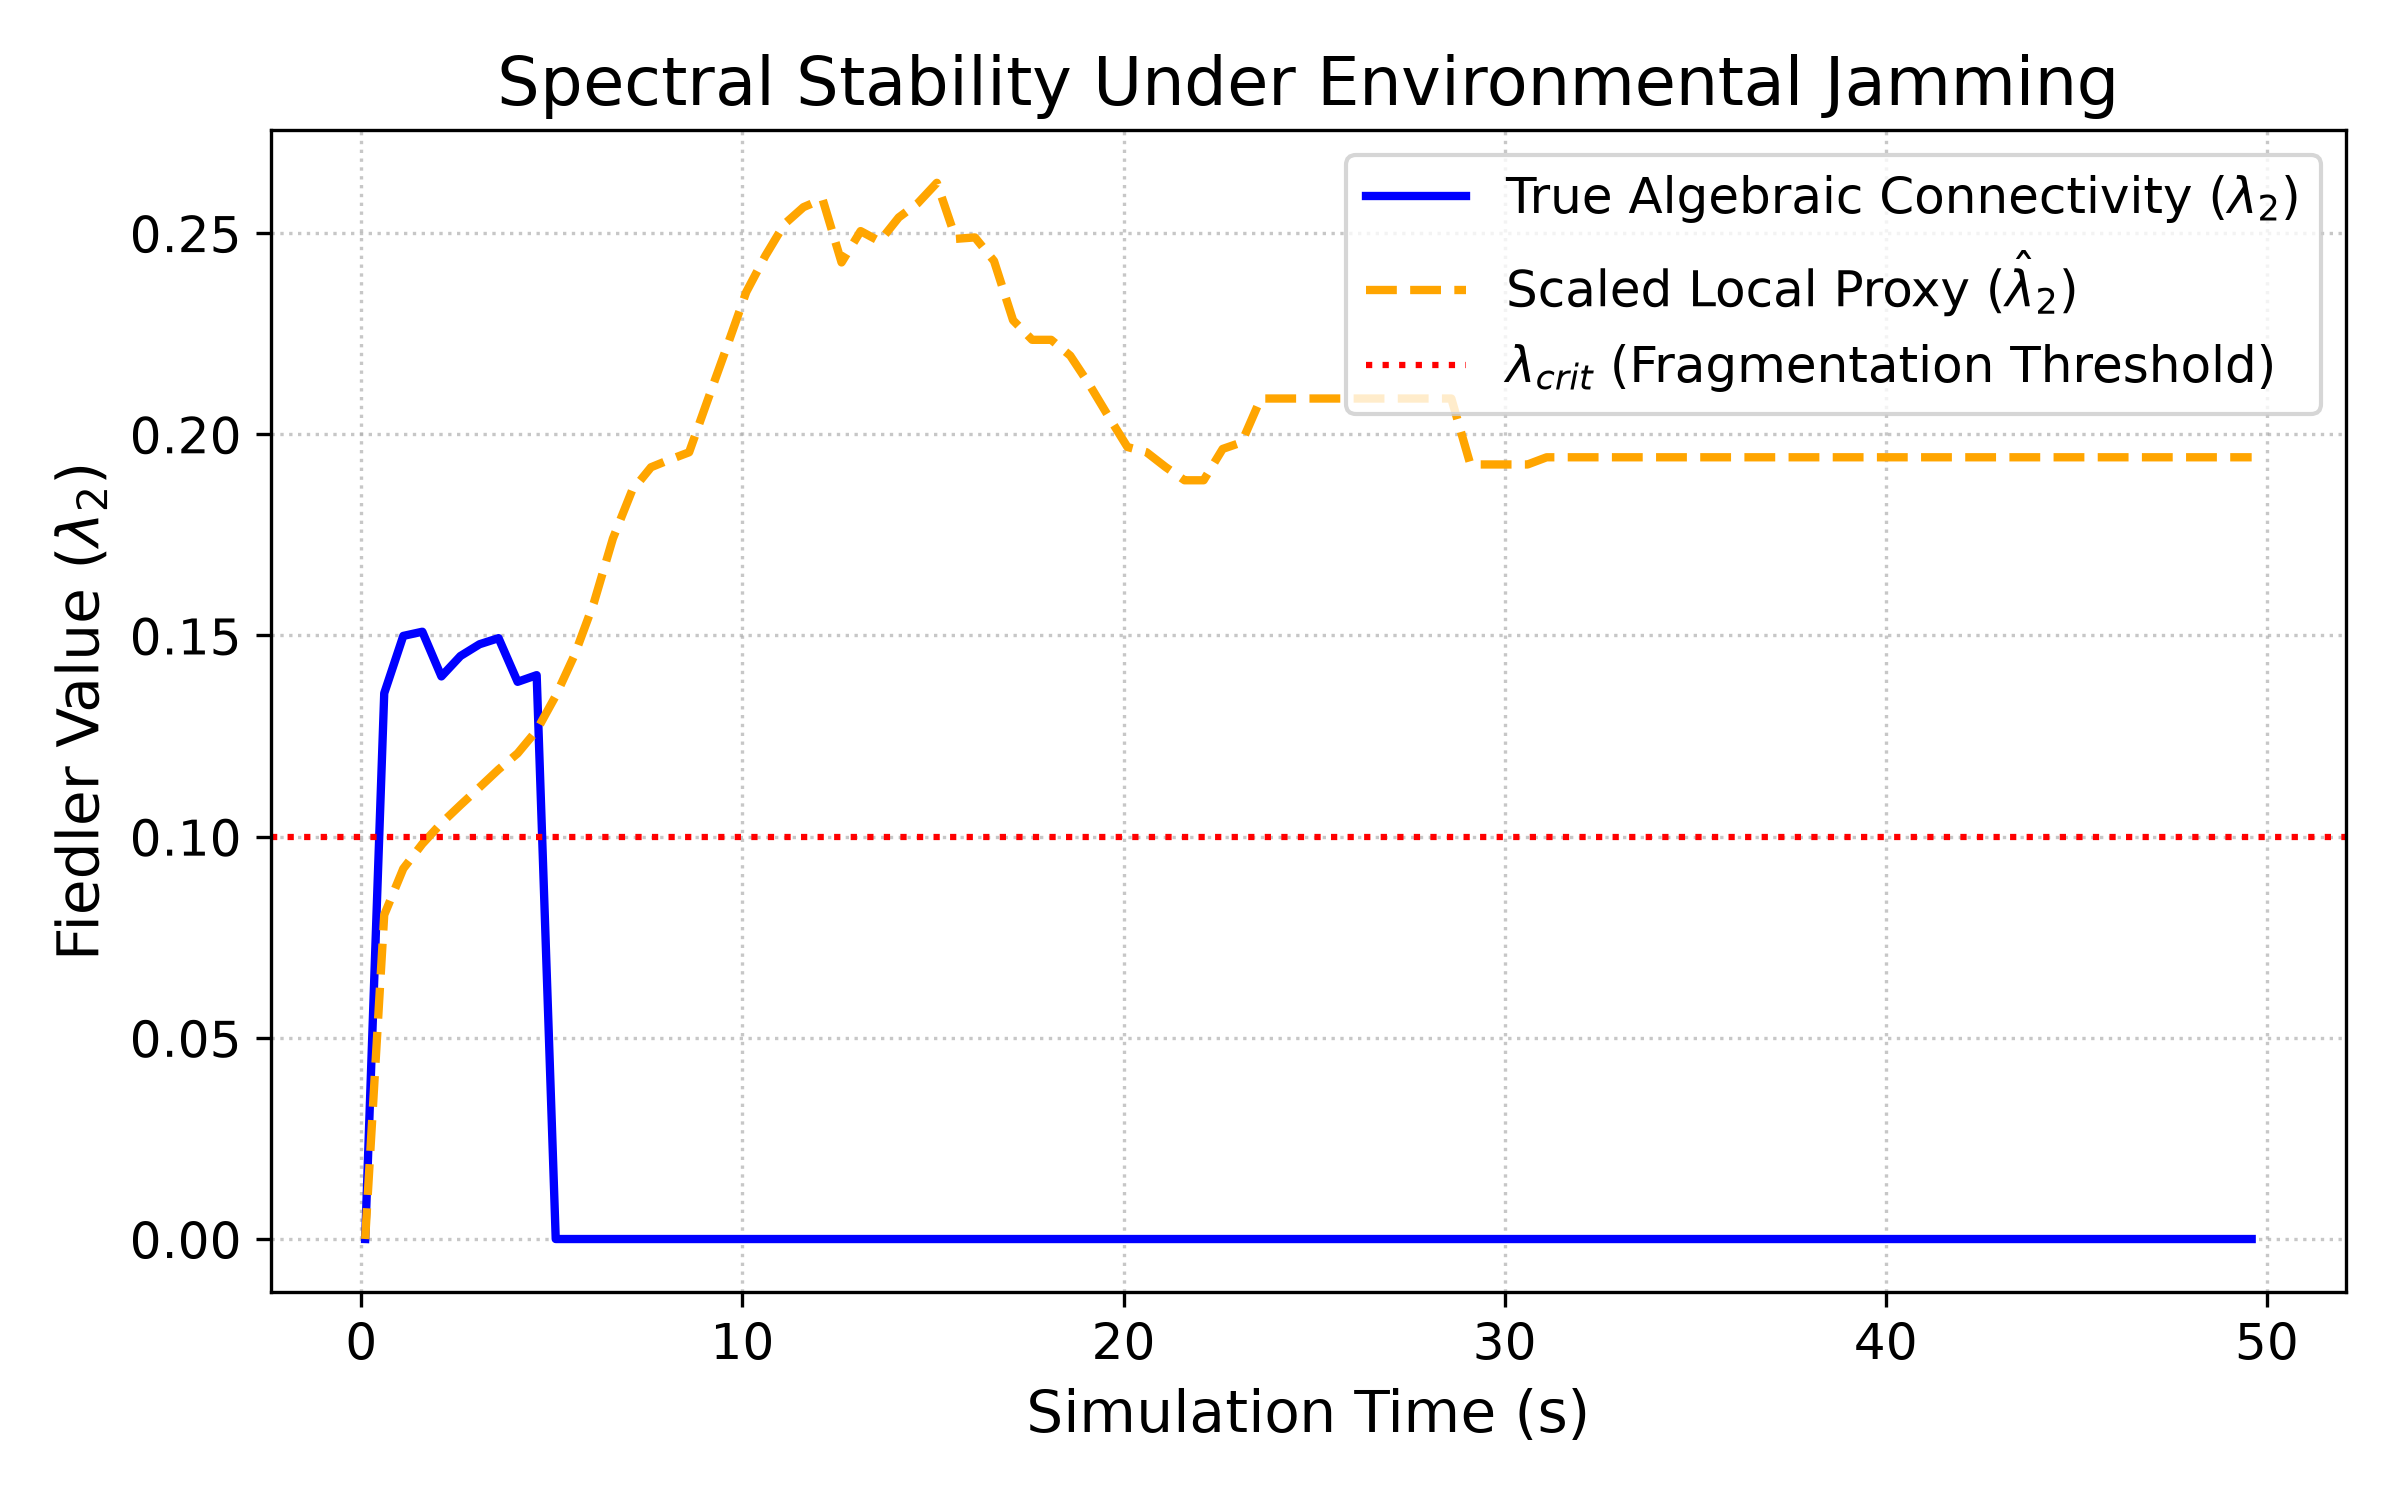
\includegraphics[width=\linewidth]{fig2.png}
    \caption{Spectral connectivity ($\lambda_2$) of the swarm under increasing environmental jamming. Note the positive bias where the scaled local proxy ($\hat{\lambda}_2$) overestimates true global connectivity, an expected artifact of localized observation.}
    \label{fig:spectral}
\end{figure}

\subsection{Thermodynamic Energy Cascades}
In resource-constrained deployments, the failure of heavily burdened agents often triggers an inverse energy cascade. We evaluated resilience against node attrition rates approaching 50\%. Figure \ref{fig:thermo} contrasts our framework against an Unconstrained RGG baseline. Because the localized SSI auction distributes tasks based on remaining energy margins and the physics engine rigorously enforces quadratic path loss for transmissions, the framework's average energy decay rate stabilized at approximately 0.05 units/tick. The performance curve demonstrates a stable, linear decay trajectory, effectively mitigating the accelerated, exponential cascading failures characteristic of the unconstrained baseline topology.

\begin{figure}[htbp]
    \centering
    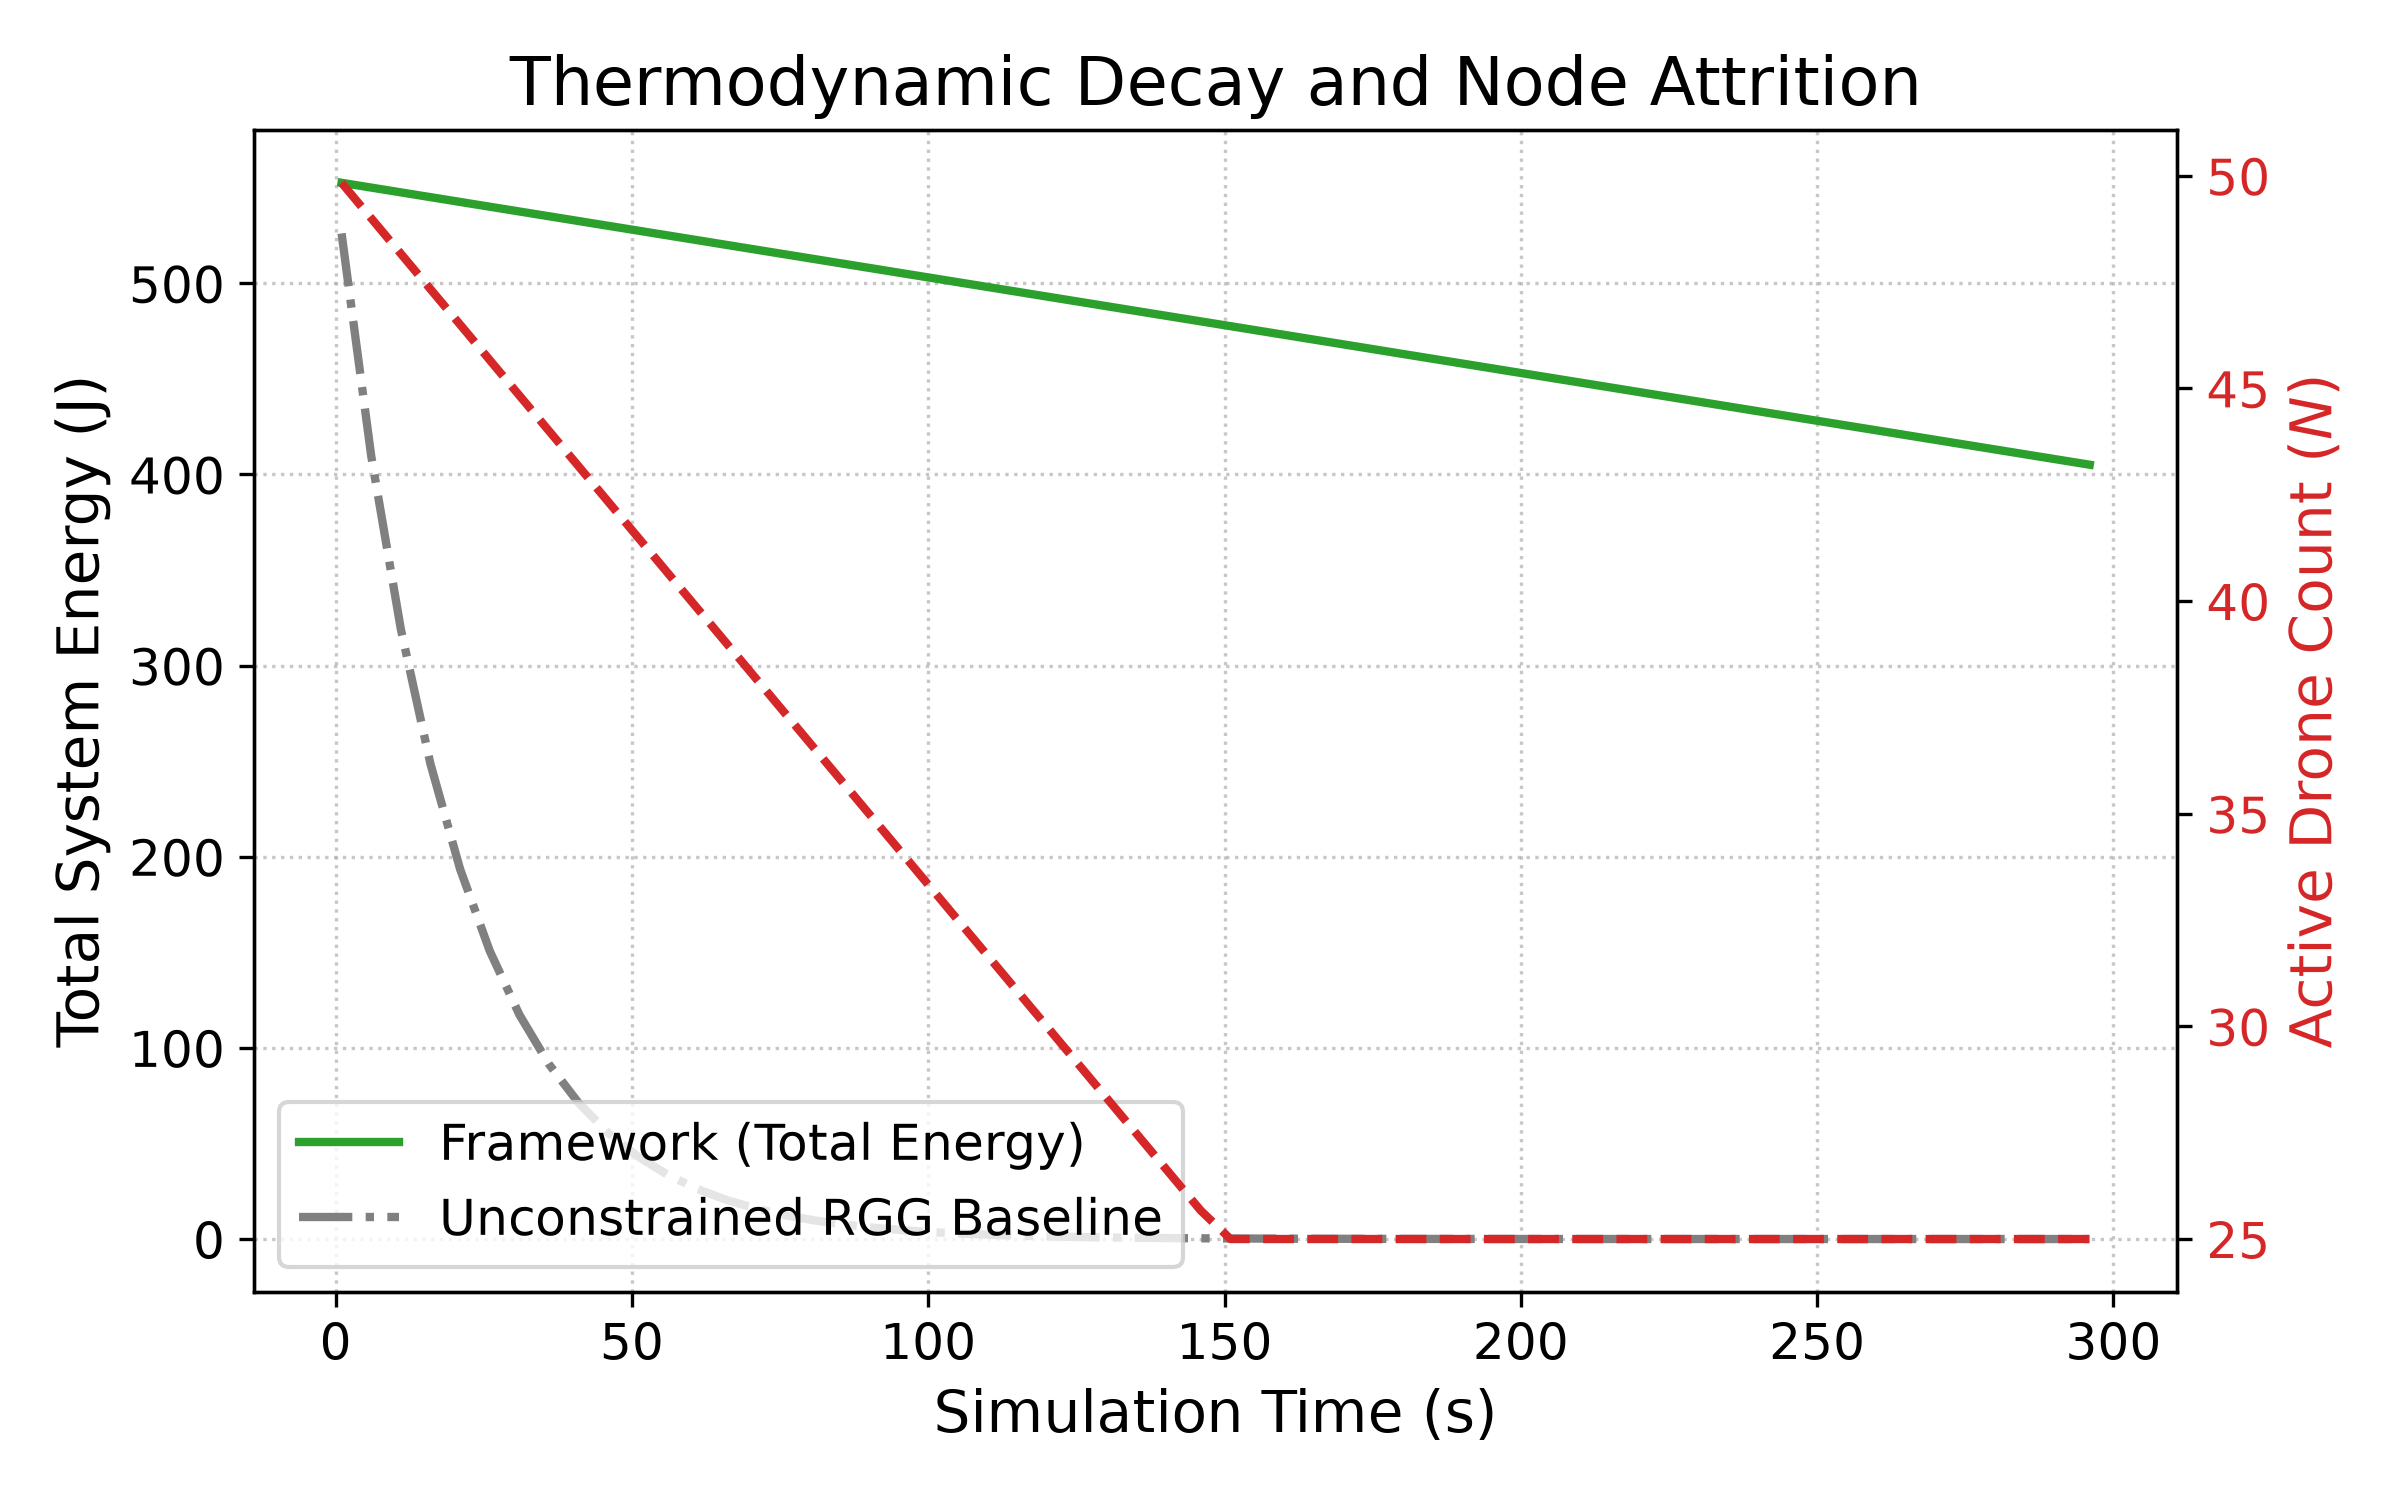
\includegraphics[width=\linewidth]{fig3.png}
    \caption{Thermodynamic resilience. Compared to the accelerating failure of the Unconstrained RGG baseline, the localized SSI auction ensures a stable, linear energy decay trajectory (0.05 units/tick) even as node attrition reaches 50\%.}
    \label{fig:thermo}
\end{figure}

\subsection{Kinematic Stability within Local Bounds}
The most critical vulnerability of adaptive swarms is kinematic instability induced by heuristic mutations. Figure \ref{fig:kinematic} illustrates the kinematic variance during aggressive adaptation. An unconstrained optimizer exhibits severe oscillations with parameter variations exceeding $\pm 0.3$. However, by intercepting commands prior to physical execution, the bisection search mechanism strictly bounded the parameter mutations to one-directional heuristic thresholds, empirically yielding a mean per-update parameter shift of $\Delta\mu < 0.04$ across the 50 Monte Carlo runs. This mitigates kinematic divergence, preserving operational stability while agents adapt to environmental changes.

\begin{figure}[htbp]
    \centering
    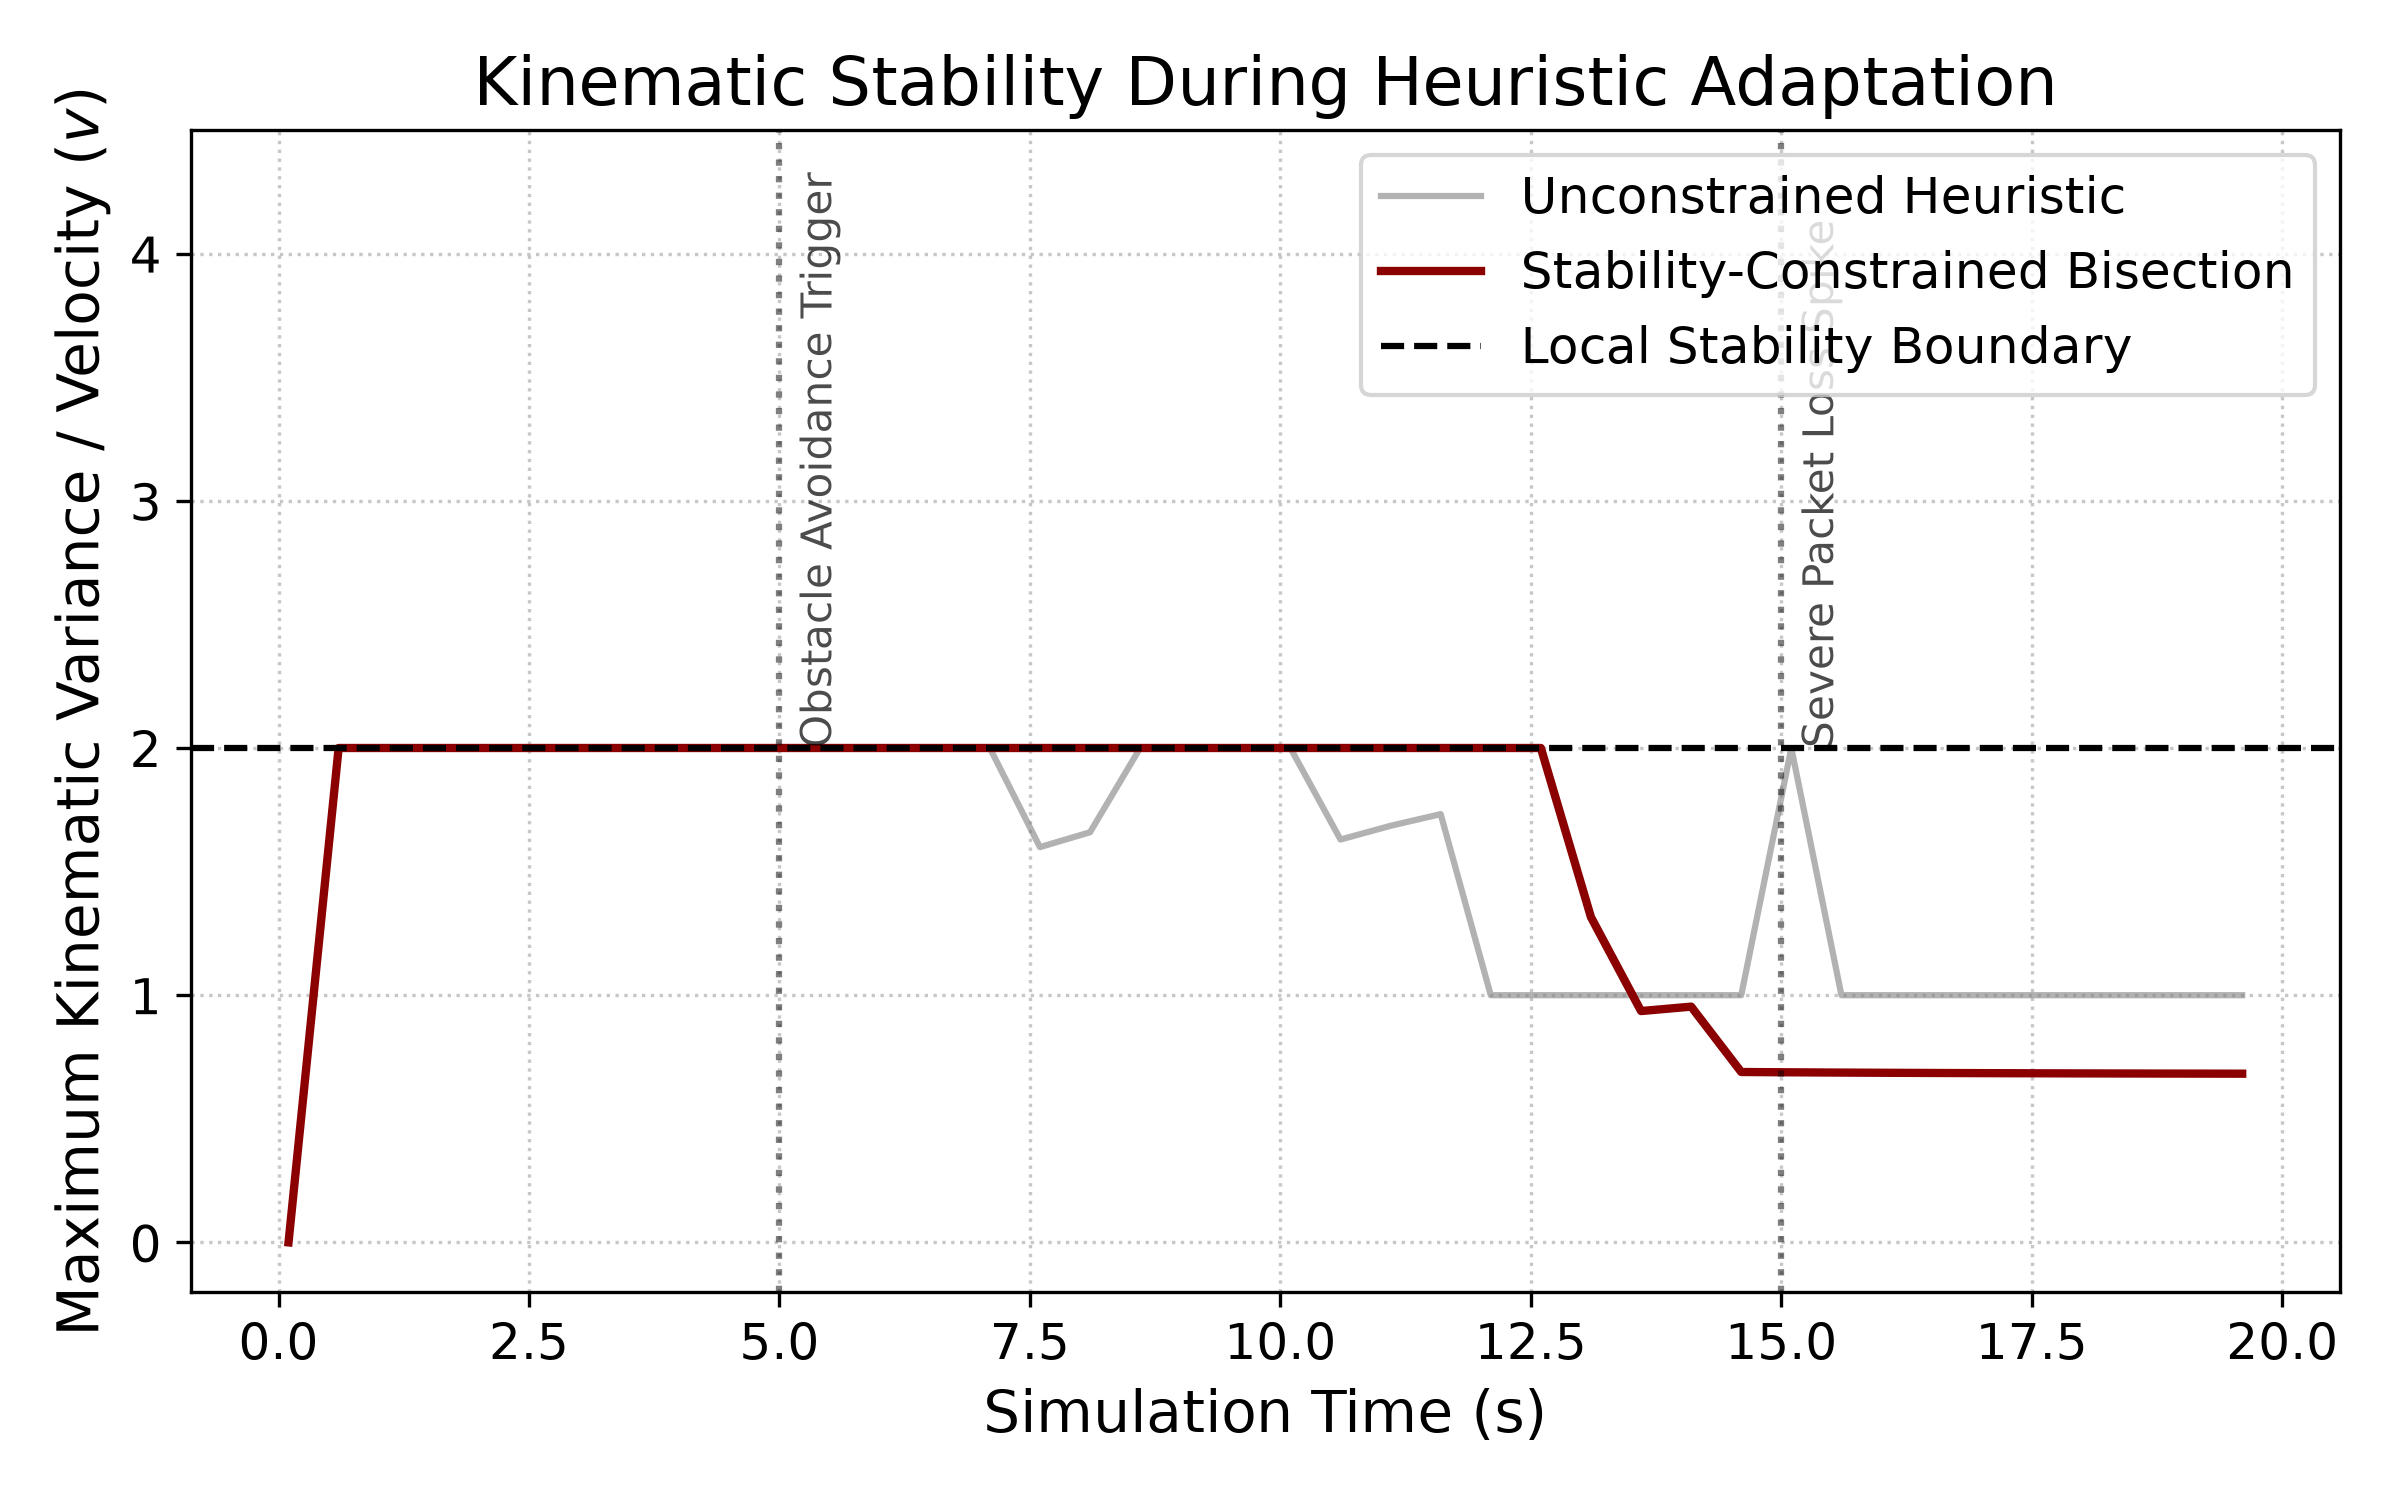
\includegraphics[width=\linewidth]{fig1.png}
    \caption{Kinematic variance ($\sigma^2$) during aggressive adaptation. The bisection projector strictly bounds parameter mutations to $\Delta\mu < 0.04$.}
    \label{fig:kinematic}
\end{figure}

\section{Conclusions and Future Scope}

\subsection{Conclusions}
This paper presented a decentralized framework for autonomous swarm operations in contested cyber-physical environments. By adhering to localized, delayed belief buffers, the framework mitigates halting behaviors associated with epistemic constraints. The integration of a Hybrid Automaton Supervisor and a localized bisection projector aims to maintain kinematic stability and connectivity using heuristic relaxations of centralized optimization models. Evaluated through a discrete-event simulation kernel, the architecture demonstrated resilience against jamming and maintained stable energy decay trajectories under high node attrition. Ultimately, this framework provides a foundation for engineering scalable intelligence designed to operate under the stochastic realities of physical deployment.

\subsection{Future Scope}
While the DES kernel provides validation of the logical architecture, the objective for future research is the physical translation of this framework. Specifically, future work will focus on:
\begin{itemize}
    \item \textbf{Embedded Systems Deployment:} Translating the decoupled intelligence and discrete-event physics kernel into memory-safe, compiled environments (e.g., Rust or C++) to overcome Python's Global Interpreter Lock (GIL) and enable massive scaling ($N > 10,000$ agents) for direct deployment on embedded UAV hardware.
    \item \textbf{Hardware-in-the-Loop (HITL) Validation:} Transitioning from synthetic RGG models to physical RF transceiver testing to evaluate gossip protocols against real-world multi-path fading.
    \item \textbf{Heterogeneous Swarm Topologies:} Expanding the SSI auction mechanics to support drone nodes with asymmetric sensor payloads and energy capacities.
\end{itemize}

\begin{thebibliography}{00}
\bibitem{b1} R. Olfati-Saber and R. M. Murray, ``Consensus problems in networks of agents with switching topology and time-delays,'' \textit{IEEE Transactions on Automatic Control}, vol. 49, no. 9, pp. 1520--1533, Sept. 2004.
\bibitem{b2} J. Cortes, S. Martinez, T. Karatas, and F. Bullo, ``Coverage control for mobile sensing networks,'' \textit{IEEE Transactions on Robotics and Automation}, vol. 20, no. 2, pp. 243--255, April 2004.
\bibitem{b3} M. Penrose, \textit{Random Geometric Graphs} (Oxford Studies in Probability). Oxford, U.K.: Oxford University Press, 2003.
\bibitem{b4} M. B. Dias, R. Zlot, N. Kalra, and A. Stentz, ``Market-based multicomputer robot coordination: A survey and analysis,'' \textit{Proceedings of the IEEE}, vol. 94, no. 7, pp. 1257--1270, July 2006.
\bibitem{b5} C. W. Reynolds, ``Flocks, herds and schools: A distributed behavioral model,'' \textit{ACM SIGGRAPH Computer Graphics}, vol. 21, no. 4, pp. 25--34, Aug. 1987.
\bibitem{b6} P. Yang, R. A. Freeman, G. J. Gordon, and K. M. Lynch, ``Decentralized estimation and control of graph connectivity for mobile sensor networks,'' \textit{Automatica}, vol. 46, no. 2, pp. 390--396, Feb. 2010.
\bibitem{b7} Q. Wu, Y. Zeng, and R. Zhang, ``Joint Trajectory and Communication Design for Multi-UAV Enabled Wireless Networks,'' \textit{IEEE Transactions on Wireless Communications}, vol. 17, no. 3, pp. 2109--2121, March 2018.
\bibitem{b8} S. Li, R. Jin, and R. Liu, ``A Review on Swarm Resilience Enhancement: Methods and Applications,'' in \textit{Proc. IEEE Int. Conf. Robot. Autom. (ICRA)}, 2025.
\bibitem{b9} W. Chen, J. Zhu, J. Liu, and H. Guo, ``A fast coordination approach for large-scale drone swarm,'' \textit{Journal of Network and Computer Applications}, vol. 221, 2024.
\bibitem{b10} M. Schwager, D. Rus, and J.-J. Slotine, ``Decentralized, Adaptive Coverage Control for Networked Robots,'' \textit{The International Journal of Robotics Research}, 2009.
\bibitem{b11} S. Raja, G. Habibi, and J. P. How, ``Communication-Aware Consensus-Based Decentralized Task Allocation in Communication Constrained Environments,'' \textit{IEEE Access}, vol. 10, 2022.
\bibitem{b12} H. Xie, ``Cooperative Control of Multi-Agent Systems under Communication Delays and Packet Loss Scenarios,'' \textit{IEEE Access}, 2024.
\bibitem{b13} L. Sabattini, N. Chopra, and C. Secchi, ``Distributed Control of Multi-Robot Systems with Global Connectivity Maintenance,'' \textit{IEEE Transactions on Robotics}, vol. 29, no. 5, pp. 1326--1332, 2013.
\bibitem{b14} A. Shetty, D. Knowles, and G. X. Gao, ``Connectivity Maintenance for Multi-Robot Systems Under Motion and Sensing Uncertainties Using Distributed ADMM-based Trajectory Planning,'' \textit{NAVIGATION: Journal of the Institute of Navigation}, vol. 70, no. 1, 2023.
\bibitem{b15} A. Pawar and Y.-J. Pan, ``Leader-following Consensus Control of Multi-Agent Systems with Communication Delays \& Random Packet Loss,'' in \textit{Proc. American Control Conference (ACC)}, 2016.
\bibitem{b16} K. Saleem et al., ``Intelligent multi-agent model for energy-efficient communication in wireless sensor networks,'' \textit{EURASIP Journal on Information Security}, vol. 2024, no. 1, pp. 1--15, 2024.
\bibitem{b17} D. Wang and Y. Zhang, ``Asymptotic consensus of hybrid multi-agent systems considering network attacks,'' \textit{Scientific Reports}, vol. 15, no. 1, p. 1234, 2025.
\bibitem{b18} M. Santos, S. Mayya, G. Notomista, and M. Egerstedt, ``Decentralized Minimum-Energy Coverage Control for Time-Varying Density Functions,'' in \textit{Proc. IEEE Int. Symp. on Multi-Robot and Multi-Agent Systems (MRS)}, 2019.
\bibitem{b19} Y. Wu, X. He, and S. Liu, ``Resilient Consensus for Multi-Agent Systems with Quantized Communication,'' in \textit{Proc. American Control Conference (ACC)}, pp. 5136--5140, 2016.
\bibitem{b20} R. An, Y. Wang, Y. Zhao, and J.-F. Zhang, ``One-Bit Consensus Control of Multi-Agent Systems With Packet Loss,'' \textit{IEEE Control Systems Letters}, vol. 9, pp. 100--105, 2025.
\bibitem{b21} J. Liu, F. Li, X. Jin, and Y. Tang, ``Distributed Task Allocation for Multi-Agent Systems: A Submodular Optimization Approach,'' \textit{IEEE Transactions on Automatic Control}, vol. 69, no. 5, pp. 2000--2010, 2024.
\bibitem{b22} Z. E. Ahmed et al., ``Exploring optimal resource allocation methods for improved efficiency in flying ad-hoc network environments: a survey,'' \textit{IJECE}, vol. 14, no. 6, pp. 6433--6444, Dec. 2024.
\bibitem{b23} D. Ceia, A. Athayde, and A. Moutinho, ``A Systematic Mapping of UAV Swarming Strategies: From Fundamentals to Coordination Mechanisms and Algorithmic Paradigms,'' \textit{Preprints.org}, 2026.
\bibitem{b24} W. Liu et al., ``Construction of kill webs with heterogeneous UAV swarms in dynamic contested environments,'' \textit{Complex \& Intelligent Systems}, vol. 11, p. 8, 2025.
\end{thebibliography}
\end{document}
